\subsubsection{Particle Swarm Optimization for Image Compression}

\paragraph{Introduction}
Particle Swarm Optimization (PSO) is a population‑based stochastic optimization algorithm inspired by the social foraging behaviour of bird flocks and fish schools, first introduced by Kennedy and Eberhart in 1995. In PSO, a swarm of particles moves through a multi‑dimensional search space, each particle representing a candidate solution. Particles adjust their trajectories based on their own experience (cognitive component) and the experience of the swarm (social component). This makes PSO particularly suitable for problems with continuous, non‑linear, and multi‑modal objective functions.

In the context of image compression, PSO can be used for colour quantisation: finding an optimal palette of $K$ colours that minimises the reconstruction error when each pixel is replaced by its nearest palette colour. This is a classic optimisation problem where the search space dimension is $K \times 3$ (each colour is an RGB triple).

\paragraph{Mathematical Formulation}
Each particle $i$ is defined by three vectors:
\begin{itemize}
    \item $\mathbf{x}_i$: current position (a candidate colour palette),
    \item $\mathbf{v}_i$: current velocity (direction and step size),
    \item $\mathbf{p}_i$: personal best position (best palette found by this particle).
\end{itemize}
The swarm also maintains a global best position $\mathbf{g}_{\text{best}}$, the best palette among all particles.

\paragraph{Fitness Function}
The quality of a palette is measured by the mean squared error (MSE) between the original image and the image reconstructed using that palette:
\[
f(\mathbf{x}) = \frac{1}{N \cdot 3} \sum_{p=1}^{N} \| \mathbf{I}_p - \mathbf{Q}(\mathbf{x}, \mathbf{I}_p) \|^2,
\]
where $N$ is the number of pixels, $\mathbf{I}_p$ is the original RGB vector of pixel $p$, and $\mathbf{Q}(\mathbf{x}, \mathbf{I}_p)$ returns the nearest colour from the palette $\mathbf{x}$. Lower MSE indicates better compression quality.

\paragraph{Personal and Global Best Update}
For each particle, the personal best is updated as:
\[
\mathbf{p}_i(t+1) = \begin{cases}
\mathbf{p}_i(t) & \text{if } f(\mathbf{x}_i(t+1)) \ge f(\mathbf{p}_i(t)),\\[4pt]
\mathbf{x}_i(t+1) & \text{if } f(\mathbf{x}_i(t+1)) < f(\mathbf{p}_i(t)).
\end{cases}
\]
The global best is then:
\[
\mathbf{g}_{\text{best}} = \arg\min_{\mathbf{p}_i} f(\mathbf{p}_i).
\]

\paragraph{Velocity and Position Update}
The velocity of each particle is updated using the canonical PSO equation:
\[
\mathbf{v}_i(t+1) = w \cdot \mathbf{v}_i(t) + c_1 r_1 \bigl(\mathbf{p}_i(t) - \mathbf{x}_i(t)\bigr) + c_2 r_2 \bigl(\mathbf{g}_{\text{best}} - \mathbf{x}_i(t)\bigr),
\]
where:
\begin{itemize}
    \item $w$ is the inertia weight (controls exploration/exploitation trade‑off),
    \item $c_1$ and $c_2$ are acceleration constants (cognitive and social components),
    \item $r_1, r_2 \sim \mathcal{U}(0,1)$ are random numbers.
\end{itemize}
The position is then updated as:
\[
\mathbf{x}_i(t+1) = \mathbf{x}_i(t) + \mathbf{v}_i(t+1).
\]

Typical parameter values used in this study are: $w = 0.7$, $c_1 = c_2 = 1.5$, swarm size $= 30$, and maximum iterations $= 50$.

\paragraph{Algorithm Pseudo‑code}
\begin{verbatim}
1. Initialize:
   For each particle i:
       Randomly initialise position x_i (palette) and velocity v_i
       Set personal best p_i = x_i
2. While iteration < max_iter and not converged:
   For each particle i:
       Reconstruct image using palette x_i
       Compute fitness f(x_i) (MSE)
       If f(x_i) < f(p_i): p_i = x_i
       Update global best g_best = argmin f(p_i)
   For each particle i:
       Update velocity v_i using PSO equation
       Update position x_i = x_i + v_i
       Clip positions to [0,255]
3. Return g_best as the optimal palette
\end{verbatim}


\begin{figure}[H]
    \centering
    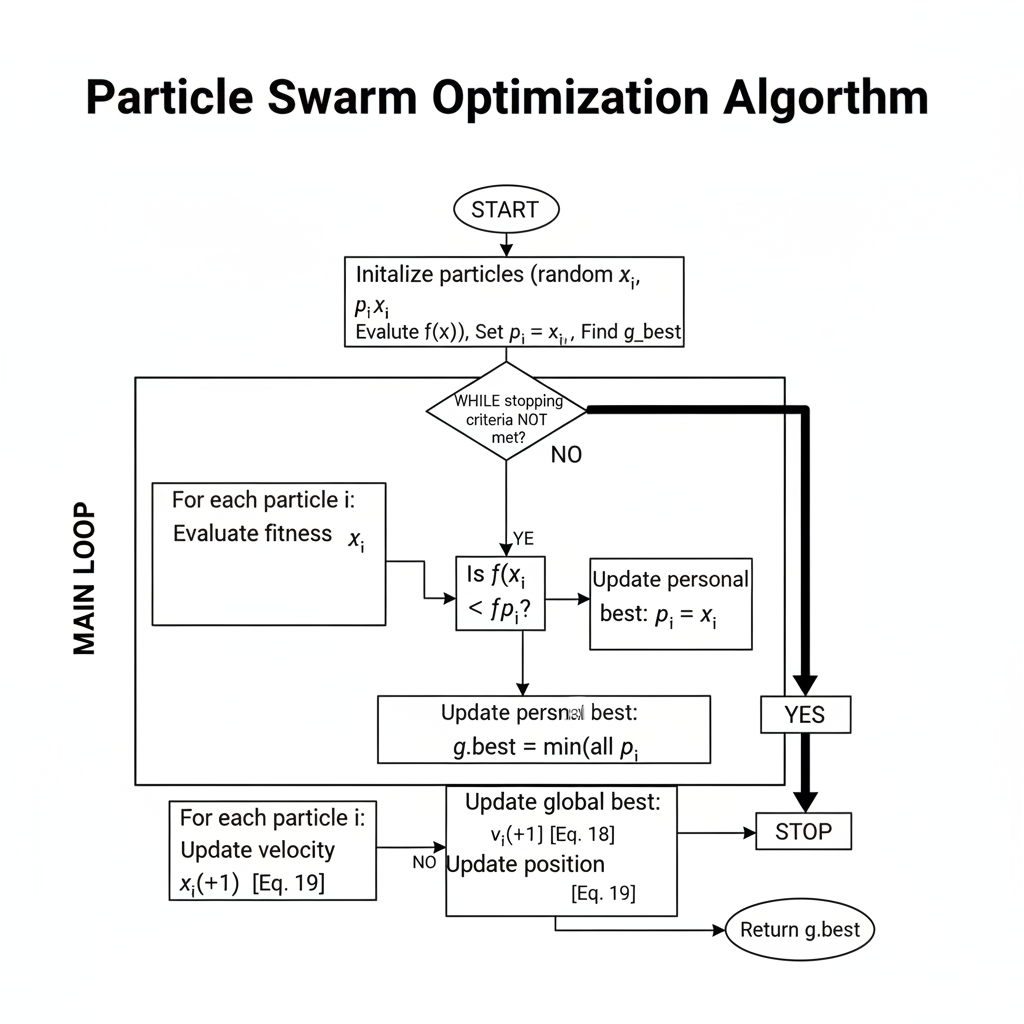
\includegraphics[width=1.0\textwidth]{pso_algo.png}
    \caption{PSO Algorithm flowchart: initialisation, fitness evaluation, personal/global best update, velocity and position update, and convergence.}
    \label{fig:pso_compression_algorithm}
\end{figure}


\paragraph{Experimental Setup}
The algorithm was implemented in Python using NumPy for vectorised operations. The standard $256\times256$ RGB Lenna image was used as the test image. Different numbers of colours $K = 4, 8, 16, 32, 64$ were evaluated. For each $K$, PSO was run with $30$ particles for $50$ iterations. The compression ratio is calculated as:
\[
\text{Ratio} = \frac{\text{Original bits}}{\text{Palette bits} + \text{Index bits}},
\]
where original bits $= 256\times256\times3\times8$, palette bits $= K\times3\times8$, and index bits $= 256\times256\times\lceil\log_2 K\rceil$.

\paragraph{Results}
Table~\ref{tab:pso_performance} summarises the performance for different $K$. The MSE decreases as $K$ increases, at the cost of a lower compression ratio and longer computation time.




\begin{table}[H]
\centering
\small
\caption{PSO compression performance on Lenna for different colour counts.}
\label{tab:pso_performance}
\begin{tabularx}{\textwidth}{|c|c|X|X|X|}
\hline
\textbf{Colours $K$} & \textbf{Compression Ratio} & \textbf{Best MSE} & \textbf{Time (s)} & \textbf{Iterations} \\
\hline
4  & 11.991:1 & 420.58 & 3.03 & 30 \\
8  & 7.992:1  & 190.74 & 5.16 & 30 \\
16 & 5.991:1  & 186.75 & 10.29 & 30 \\
32 & 4.789:1  & 140.49 & 19.85 & 30 \\
64 & 3.984:1  & 105.79 & 38.92 & 30 \\
\hline
\end{tabularx}
\end{table}

For a more detailed analysis, PSO was run again with $K=16$, $30$ particles, and $50$ iterations. The convergence behaviour is shown in Table~\ref{tab:pso_convergence} and Figure~\ref{fig:pso_convergence}.



\begin{table}[H]
\centering
\caption{PSO convergence history for $K=16$.}
\label{tab:pso_convergence}
\begin{tabular}{|c|c|}
\hline
\textbf{Iteration} & \textbf{Best MSE} \\
\hline
0   & 585.49 \\
10  & 230.20 \\
20  & 166.22 \\
30  & 152.82 \\
40  & 135.32 \\
49  & 126.80 \\
\hline
\end{tabular}
\end{table}

The final compressed image achieved an MSE of $126.80$ and a compression ratio of $5.991:1$. The actual storage breakdown is:

\begin{table}[H]
\centering
\caption{Storage breakdown for PSO compression ($K=16$).}
\label{tab:pso_storage}
\begin{tabularx}{\textwidth}{|l|X|}
\hline
\textbf{Component} & \textbf{Size} \\
\hline
Original image & 192.00 KB (196,608 bytes) \\
Palette ($16\times3$ bytes) & 48 bytes \\
Index map ($65536$ pixels $\times$ 4 bits) & 32,768 bytes \\
Total compressed & 32,816 bytes (32.05 KB) \\
\hline
\textbf{Compression ratio} & \textbf{5.991:1} \\
\textbf{Space saved} & 83.3\% \\
\hline
\end{tabularx}
\end{table}

\paragraph{Comparison with K‑Means}
The same image was compressed using a custom K‑Means implementation ($K=16$). Table~\ref{tab:pso_vs_kmeans} compares the two methods.

\begin{table}[H]
\centering
\caption{Comparison of PSO and K‑Means for colour quantisation ($K=16$).}
\label{tab:pso_vs_kmeans}
\begin{tabular}{l c c}
\hline
\textbf{Metric} & \textbf{PSO} & \textbf{K‑Means} \\
\hline
Compression ratio & 5.991:1 & 5.991:1 \\
MSE & 126.80 & — \\
PSNR (dB) & 27.1 & — \\
Time (s) & 24.84 & 0.64 \\
\hline
\end{tabular}
\end{table}

PSO achieves a lower MSE (better quality) than K‑Means when both use the same number of colours, but at a significantly higher computational cost. This trade‑off is typical: PSO explores the search space more thoroughly, while K‑Means converges quickly to a local optimum.

\paragraph{Visual Analysis}
Figure~\ref{fig:pso_compression_visuals} (to be inserted) shows:
\begin{itemize}
    \item Original Lenna image.
    \item Compressed images for $K=4,8,16,32,64$.
    \item Error map for $K=16$ (brighter regions indicate larger reconstruction error).
    \item The optimised colour palette (16 colours).
    \item PSO convergence curve (MSE vs. iteration).
\end{itemize}

Figure~\ref{fig:pso_vs_kmeans} (to be inserted) provides a side‑by‑side comparison of the compressed images and error maps from PSO and K‑Means.

\paragraph{Discussion}
\begin{itemize}
    \item \textbf{Quality vs. Compression:} Increasing $K$ improves image quality (lower MSE) but reduces the compression ratio. For $K=16$, the ratio $5.99:1$ offers a good balance.
    \item \textbf{Convergence:} The MSE drops rapidly in the first 10 iterations and then slowly improves, demonstrating that PSO effectively explores the search space.
    \item \textbf{Comparison with K‑Means:} PSO produces higher quality (lower MSE) at the cost of longer computation. For applications where quality is paramount and offline processing is acceptable, PSO is advantageous; for real‑time applications, K‑Means remains preferable.
    \item \textbf{Parameter sensitivity:} The chosen parameters ($w=0.7$, $c_1=c_2=1.5$) gave stable convergence. A decreasing inertia weight could further improve final accuracy.
\end{itemize}

\paragraph{Summary}
Particle Swarm Optimization is an effective metaheuristic for colour quantisation in lossy image compression. It finds near‑optimal palettes by balancing individual and collective knowledge. Experimental results on the Lenna image show that PSO achieves compression ratios from $12:1$ ($K=4$) to $4:1$ ($K=64$) while minimising reconstruction error. Compared to K‑Means, PSO yields better image quality at the expense of higher computational cost. The flexibility of PSO allows easy adaptation to other compression‑related optimisation problems, such as codebook design in vector quantisation or transform coefficient selection.

\begin{figure}[H]
    \centering
    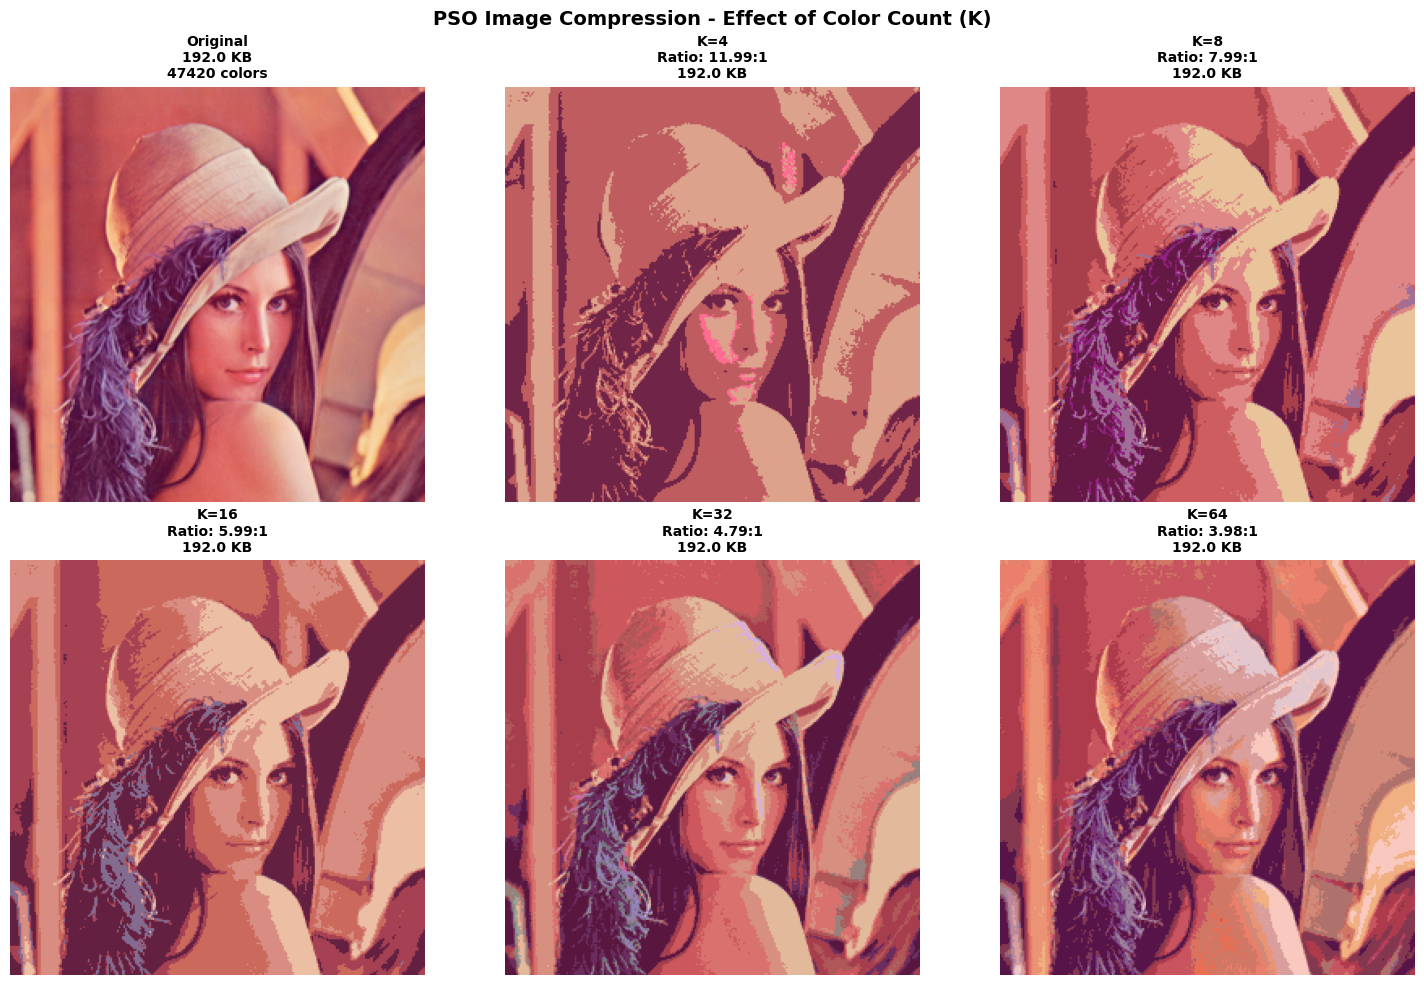
\includegraphics[width=1.0\textwidth]{pso_compare.png}
    \caption{PSO compression results: (a) original Lenna, (b)–(f) compressed with $K=4,8,16,32,64$, (g) error map for $K=16$, (h) colour palette, (i) convergence curve.}
    \label{fig:pso_compression_visuals}
\end{figure}


\begin{figure}[H]
    \centering
    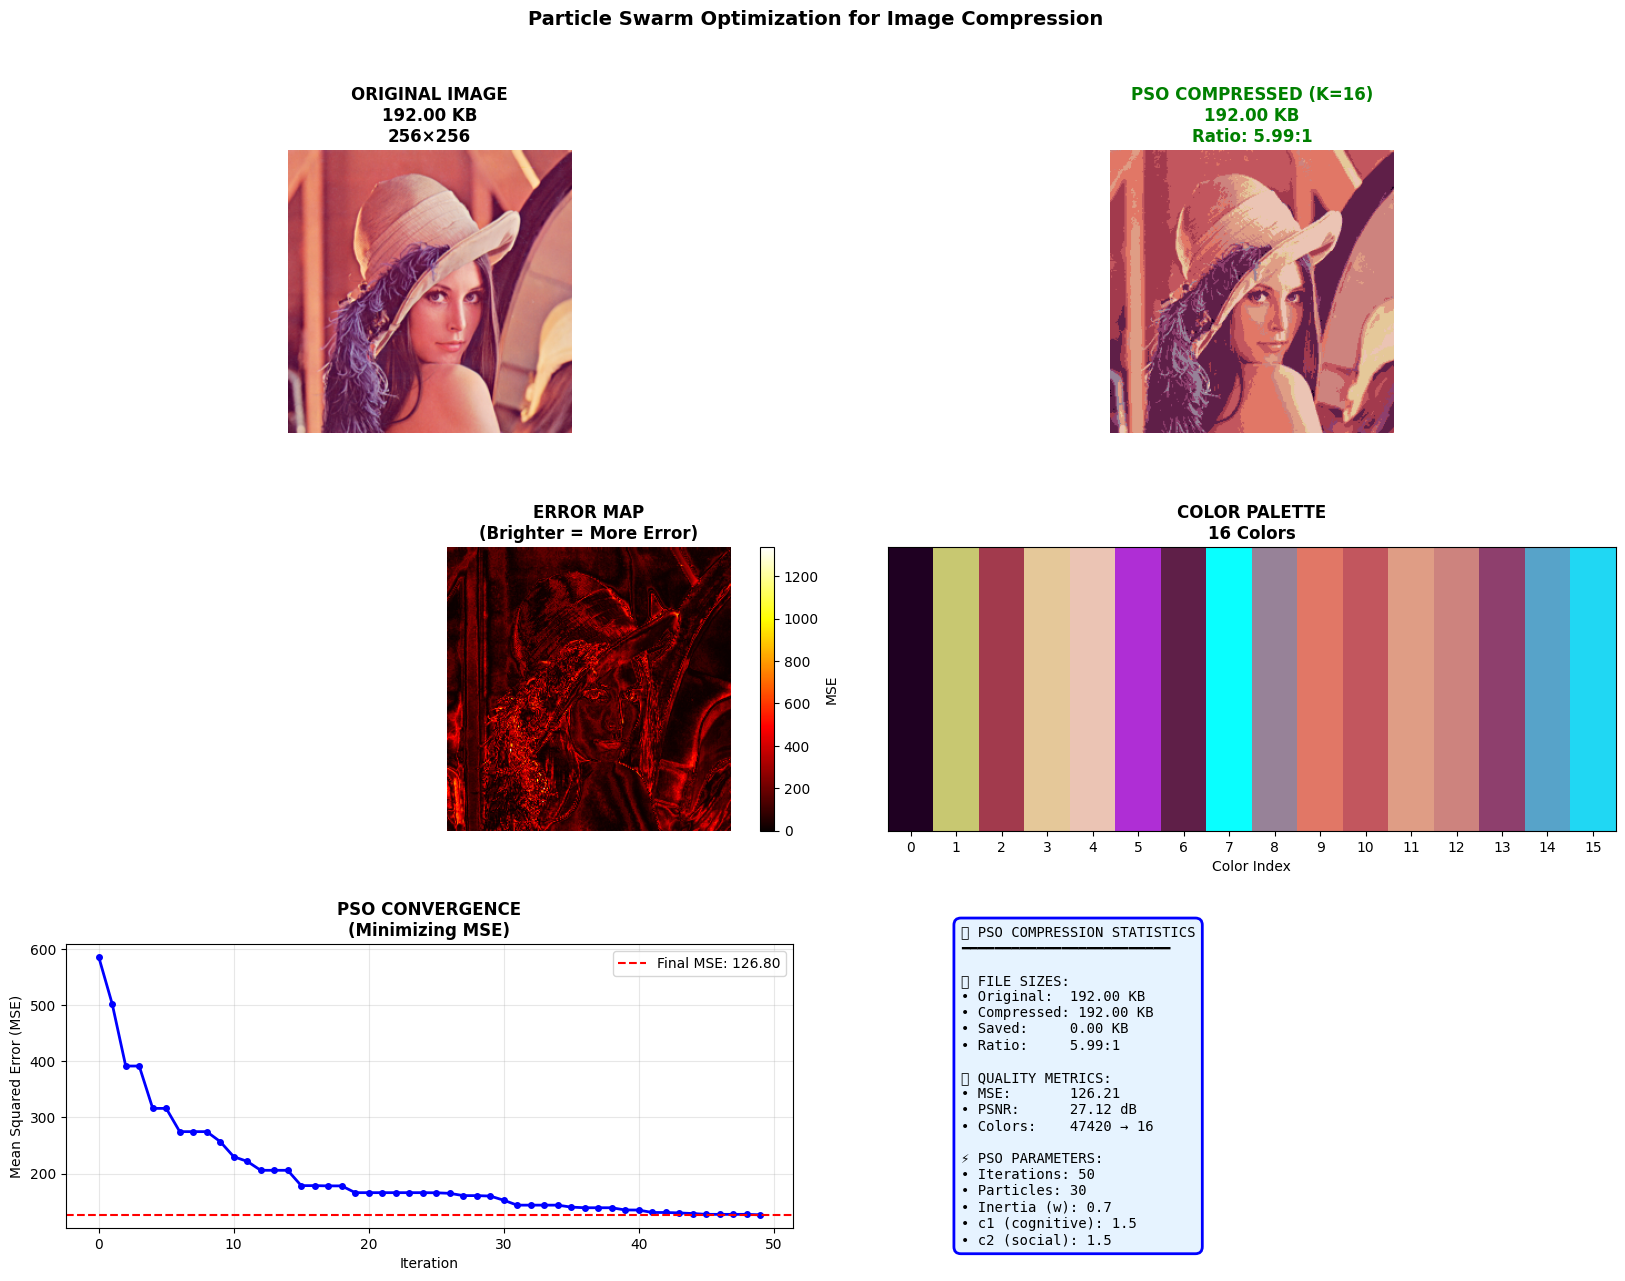
\includegraphics[width=1.0\textwidth]{pso_opti.png}
    \caption{PSO convergence comparison: (a) MSE vs. iteration for PSO, (b) MSE vs. iteration for K‑Means.}
    \label{fig:pso_optimization_comparison}
\end{figure}

\begin{figure}[H]
    \centering
    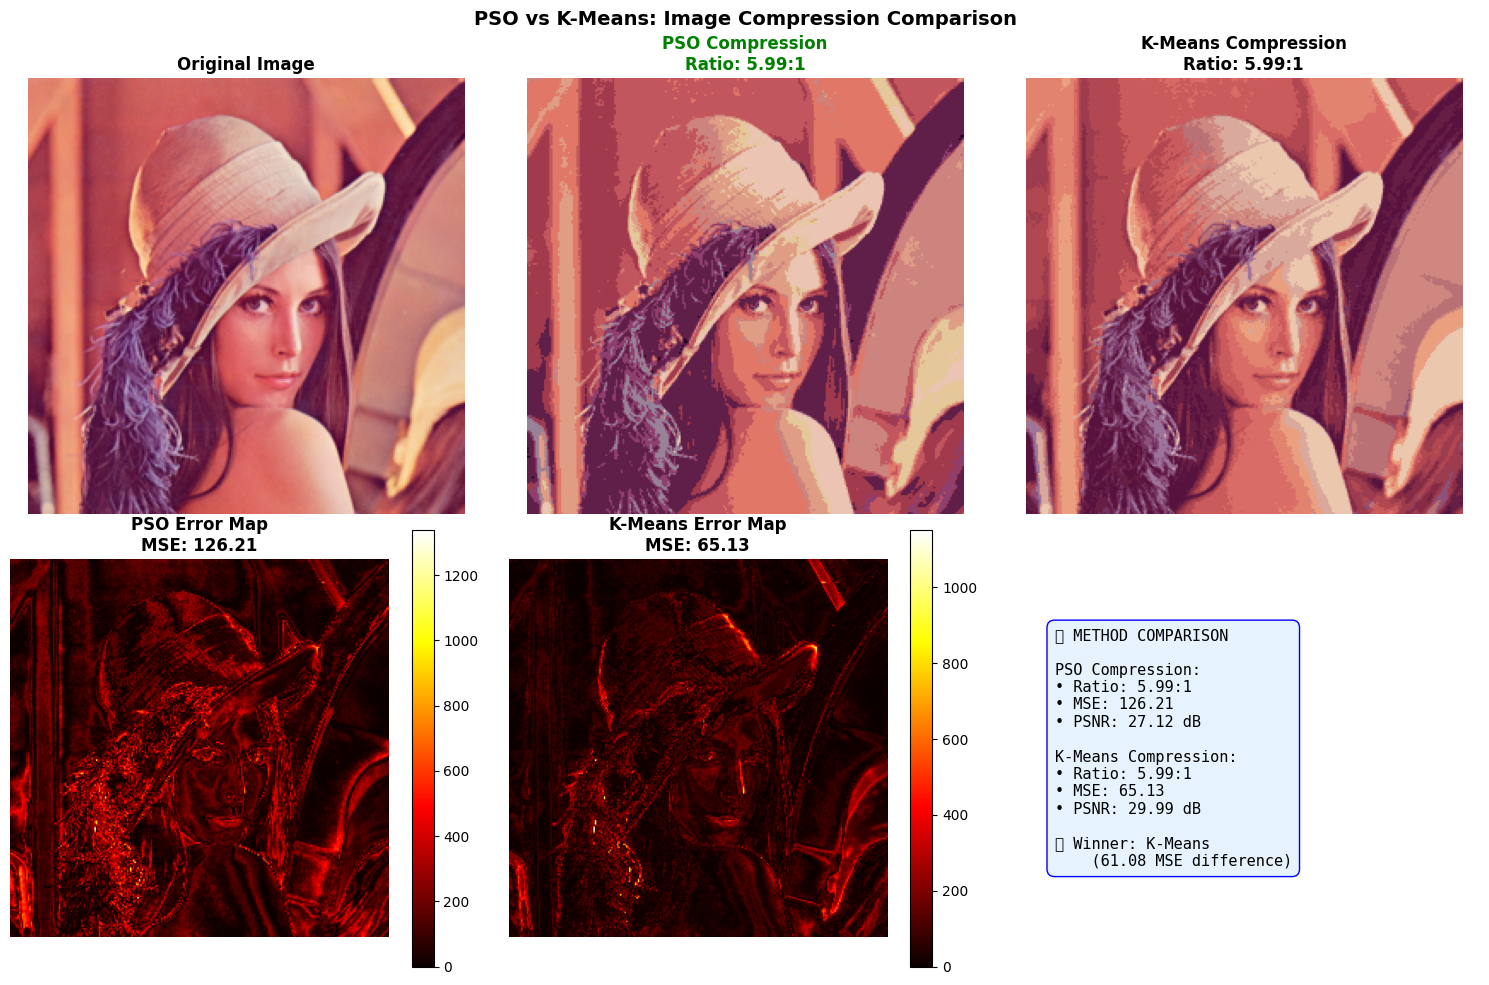
\includegraphics[width=1.0\textwidth]{pso_kmean.png}
    \caption{Comparison between PSO and K‑Means for $K=16$: (a) PSO compressed, (b) K‑Means compressed, (c) PSO error map, (d) K‑Means error map.}
    \label{fig:pso_vs_kmeans}
\end{figure}

